\section{Application Scenarios}
\label{sec:scenarios}
%
Our obstruction-free fish-eye lens can be used with different types of volumetric datasets. To illustrate this, we next present four such use-cases considering scalar density volumes coming from baggage inspection, 3D flow simulation, radiology, and air traffic management.

\subsection{Baggage inspection: An unusual blunt object}
\label{sec:baggage}
%
\begin{figure*}[htbp]
\includegraphics [width=\textwidth]{images/aircraft_lens.pdf} 
\caption{Inspecting an abnormal aircraft trajectory. (a) The initial view on the trajectories where the abnormal trajectory was spotted. (b) The transition  towards a magnified trajectory starts just after the lens tool has been used (double click). (c) The trajectories is magnified. (d) Local Rotations allow to look around the target (right click+ mouse drag toward the desired direction).}
\label{f:aircraft_lens}
\end{figure*}
%
In most airports, security agents deal with volumetric data exploration during baggage inspections. While automatic systems are now able to detect densities of harmful substances such as C-4, TNT, and nitroglycerin, and event some prohibited articles such as classical firearms and knives, it remains difficult to identify unusual threats. In addition, baggage inspection faces four main concealment strategies\,\cite{xxx}:

\vspace{0.15cm}
\noindent\textbf{Superposition}: A threat (prohibited object) may be sheltered among dense materials. It is sometimes possible to see through such a `shield' using high penetration (enhanced X-ray power) or image processing (contrast improvement) techniques. However, such techniques are not universally available and also require fine-tuning various parameters, which slows down the inspection process.

\vspace{0.15cm}
\noindent\textbf{Location}: Depending on its location inside the luggage, a threat can be hard to detect. Objects located in the corners, edges, or in the luggage’s frame are very hard to spot.

\vspace{0.15cm}
\noindent\textbf{Dissociation}: One can conceal a threat by spreading its parts in the luggage, \emph{e.g}, by disassembling a weapon and scattering its parts.

\vspace{0.15cm}
\noindent\textbf{Lure}: A lure can be used to to hide the real threat. For instance, a minor threat like a small scissors c be clearly visible and catch the security agent's attention while a more important threat remains hidden.

Consider the baggage scan in \autoref{f:baggage_lens} with a volume size of 283x189x344 voxels. Automatic baggage inspection systems will not detect anything suspect on this scan. However, while visually exploring this baggage from different angles (\autoref{f:baggage_lens}a-c), it appears that an object is hidden between a set of mugs. A common solution to this type of issue in baggage inspection is to filter materials by density in order to show or hide subsets of the volume and reduce the occlusion. However, in this case, this solution does not work, as the suspect target has almost the same density as the surrounding mugs. Hence, removing the occludes will also remove the target (\autoref{f:baggage_lens}d-f). Using the obstruction-free fish-eye lens helps in this kind of situation. Clicking on the sharp detail visible in \autoref{f:baggage_lens}c first gathers rays so they pass through the low-density zone between the mugs (\autoref{f:baggage_lens}f)

The user has just to use this tool on the partially hidden target. Then, a transition inside the lens will start and smoothly provide the finale unobstructed view of the blunt object which is, in this case, a ceramic shuriken (\autoref{f:baggage_lens}e-g). However, this shows only a small part of the target. Scattering rays next fully reveals the target (\autoref{f:baggage_lens}h). The user can adjust the lens size to get a more detailed view of the target (\autoref{f:baggage_lens}i). From this view, the controller decides that the target is a copy of a shuriken (Japanese ninja star weapon).

\subsection{Fluid flow: A deep-buried spherical vortex}
\label{sec:flow}
%
%
Flow visualization using streamlines has a long history in scientific visualization~\cite{brambilla2012illustrative,xxx}. When applied to 3D datasets, a key challenge is to balance the streamline density. Low values allow seeing inner regions in the data but can subsample (miss) important patterns. High values show more data but create too much occlusion. We next show how our lens can be used to discover interesting patterns in the second case, \emph{i.e.}, a 3D volume densely filled with streamlines. The dataset, introduced in\,\cite{griebel2004flow}, captures the simulation of water flow in a basin computed on a grid of 128x85x42 cells. A set of 4595 streamlines with 183K sample points is next traced by pseudo-random seeding over this vector field. We convert this set of 3D curves (polylines) to a scalar volume by using kernel density estimation (KDE)\,\cite{silverman1986density}. Similar techniques have been used to compute density maps of 2D trail-sets\,\cite{hurter2012graph,cubu,hurter2015image}. To increase computational speed, we compute the KDE in the frequency space and using GPU acceleration, following\,\cite{lhuillier2017ffteb}. The resulting volumes have a resolution of $500^3$ voxels and can be directly displayed using DVR (\autoref{f:stream_lens}). Note that, given the smoothing effect of KDE, streamlines appear now as finite-thickness tubes rather than pixel-thin curves.

For a first overview, we display the volume using standard DVR. After turning the viewpoint a bit, we notice a dense spherical item inside the dataset (\autoref{f:stream_lens}a). To see its shape better, we increase the opacity; however, this immediately increases occlusion so the item becomes invisible. Conversely, decreasing opacity to reduce occlusion makes the item almost transparent. Our lens solves the problem: In the initial view (\autoref{f:stream_lens}a), we point at the target and turn on the lens. This effectively pushes away the occluding stream bundles, and lets us see that our item is nearly perfectly spherical (\autoref{f:stream_lens}b). This is something we could not have assessed from \emph{any} viewpoint and with likely any opacity modulation using standard DVR. Our object is a set of densely-packed, low-speed, tightly-turning streamlines that create a ball-like vortex. Interestingly, this spherical vortex has not been discovered by any of the visualization techniques that we are aware of that used this same dataset\,\cite{telea_vis_99,griebel2004flow,ddh,lhuillier2017ffteb,maybe_more}. To make sure our target is spherical, we view it in the lens from different directions, by interactively changing the ray directions in the lens (\autoref{f:stream_lens}c). Finally, we can close the lens but keep the target magnified (\autoref{f:stream_lens}d).


\begin{figure*}[htb]
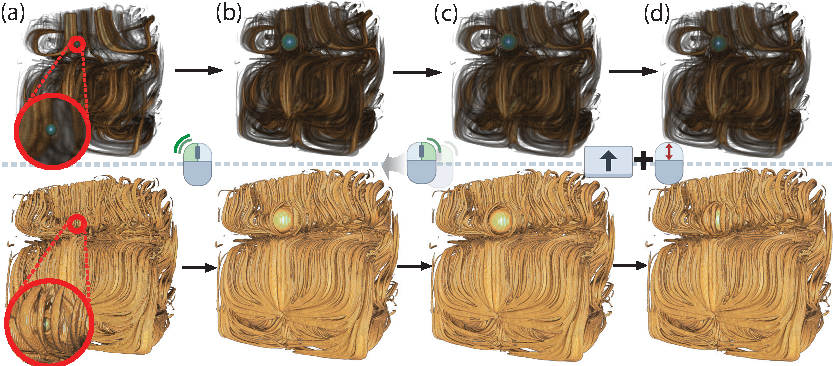
\includegraphics [width=\textwidth]{images/stream_lens.eps}
\caption{Flow volume exploration using two different opacity transfer functions (top and bottom rows). From the viewpoint (a), a small high-density spherical item appears between the streamlines. (b) The lens is applied at that location (double click). (c) The directions of rays inside the lens are changed to see the whole spherical target in the lens (right click + mouse drag change direction). (d) The lens is gradually closed while keeping the focus area magnified (shift + scroll).}
\label{f:stream_lens}
\end{figure*}

\subsection{Chest scan: A hard to see tumor}
%
In our third use-case, we consider a contrast chest CT scan (512x512x110 voxels) of an elderly patient having a sizeable (roughly 8 cm diameter) lung tumor. Typical examination of such data by the pulmonologist and radiologist in charge involves using slice-based views. In some of these views, the tumor is clearly visible (\autoref{f:slicer}a,c), though not in all of them (\autoref{f:slicer}b). Moreover, the exact tumor shape, morphology, and connection to the lung walls is not easy to assess. Using standard DVR makes the tumor partially visible (\autoref{f:slicer}d). However, occlusion from the rib cage and other tissues is still present. Using both TF presets and manually changing the TFs of the 3D Slicer tool\,\cite{slicer} used to construct the DVR could not help de-occluding the tumor without making (parts of) it transparent.

\begin{figure}[htb]
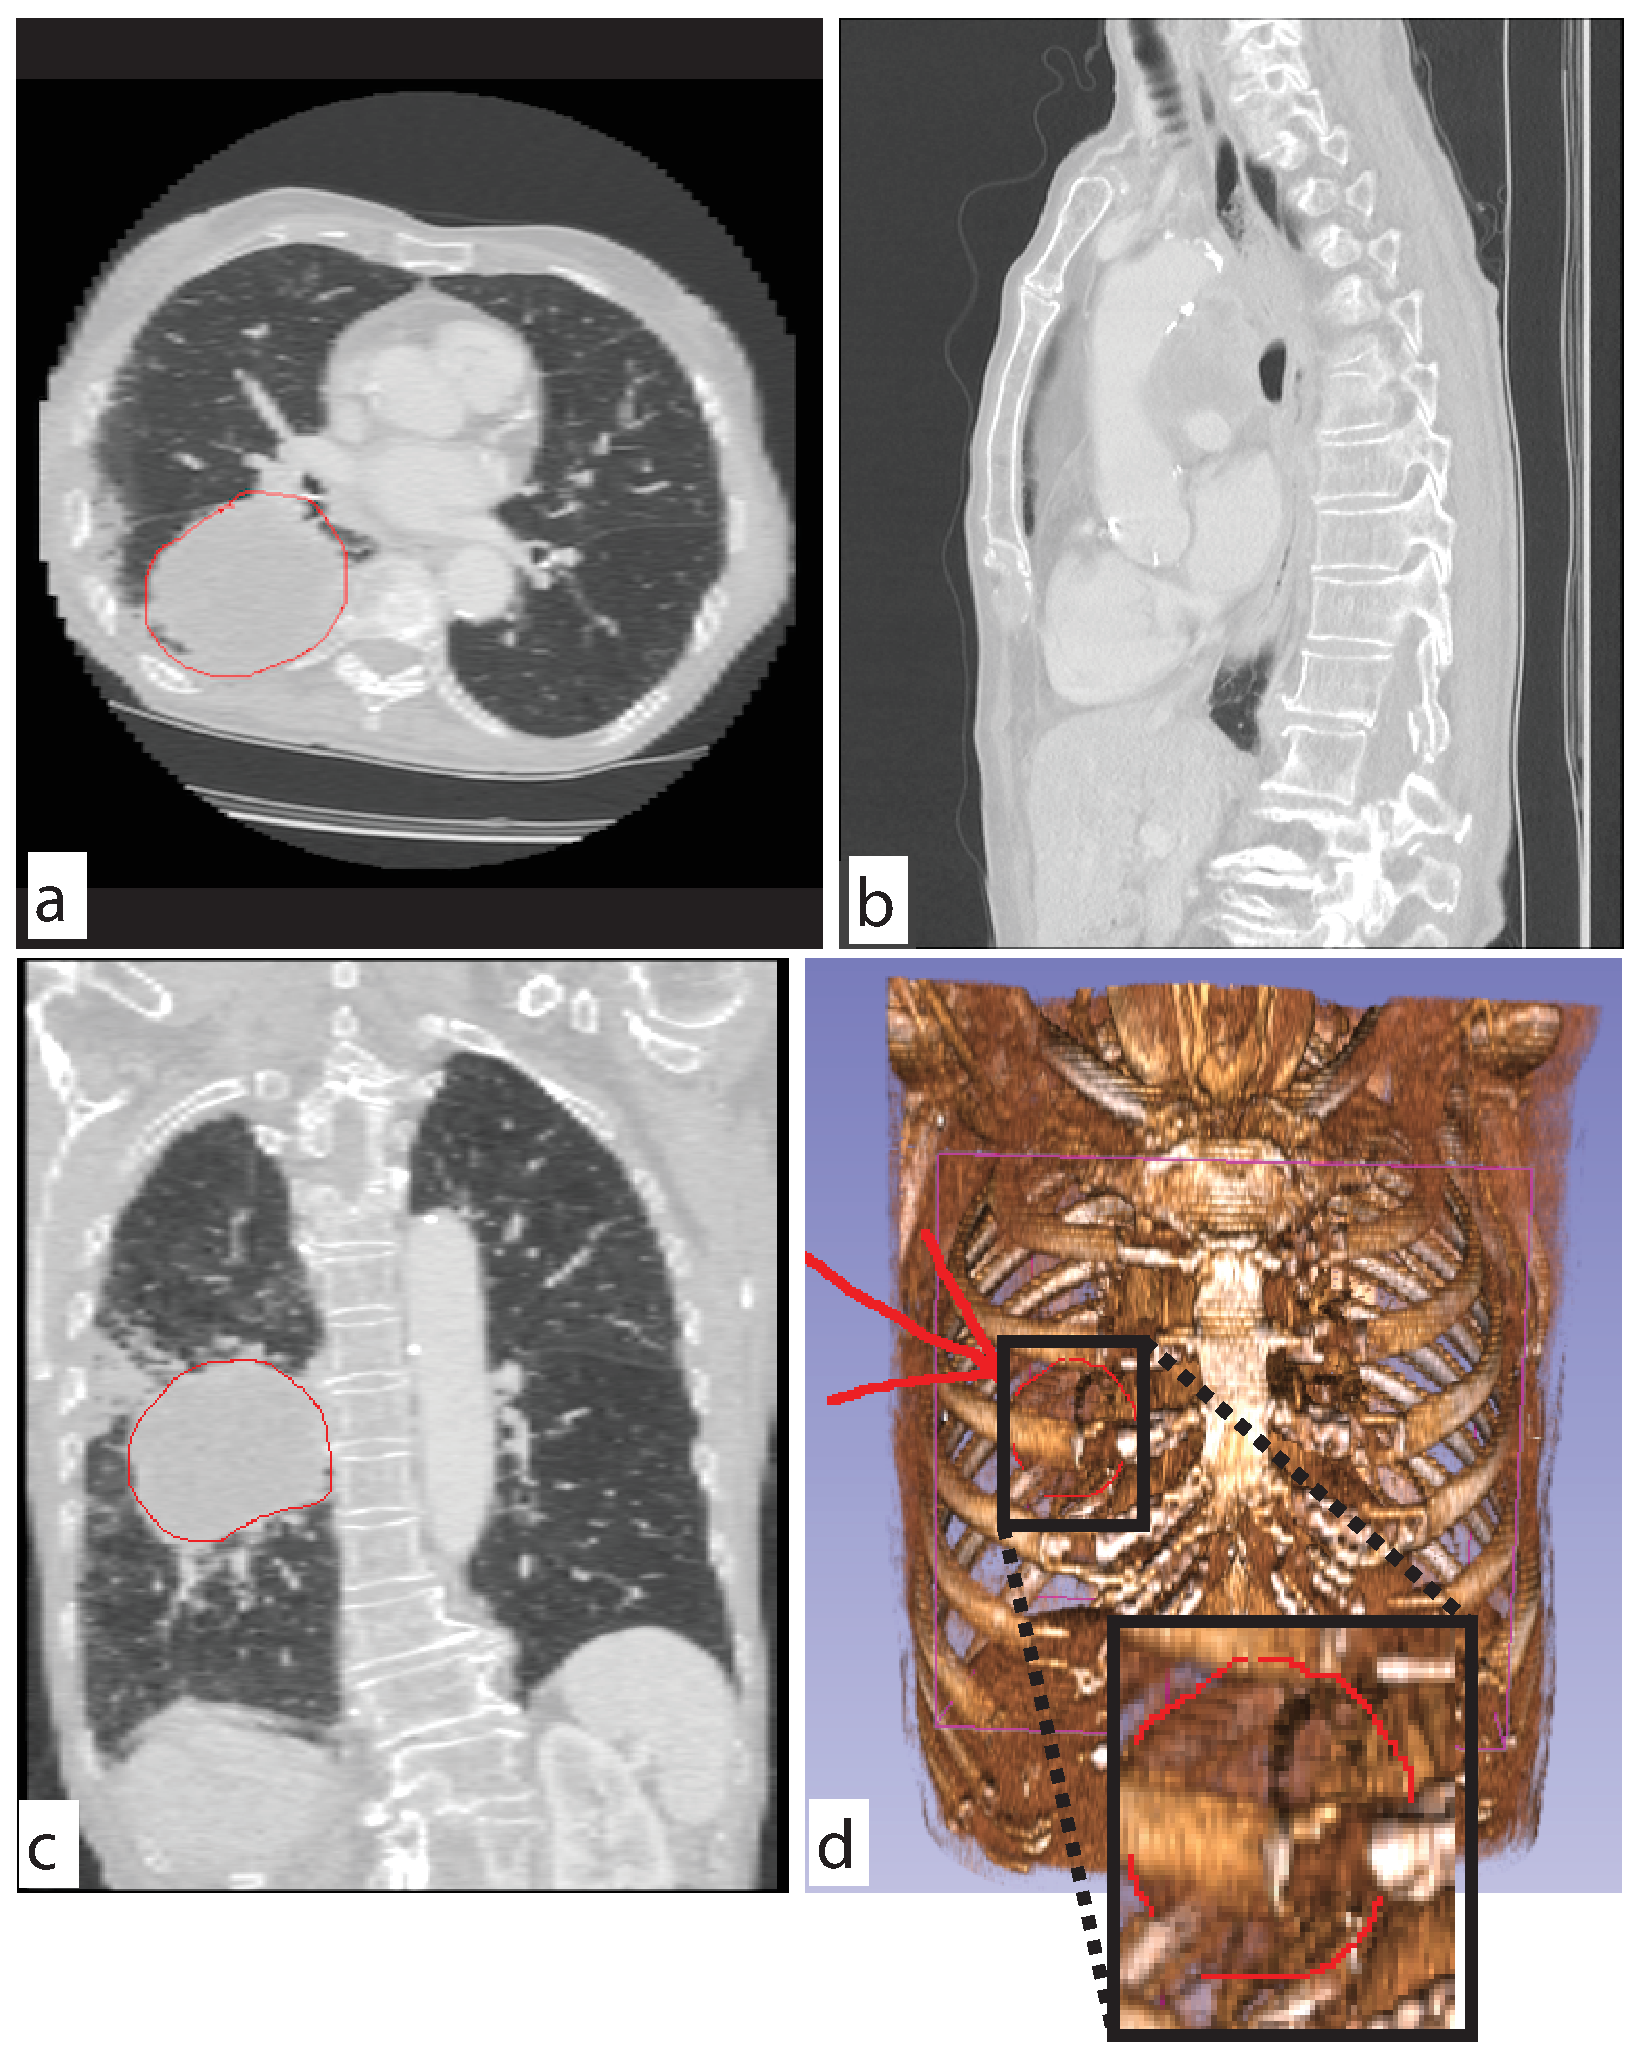
\includegraphics [width=0.48\textwidth]{images/slicer.eps}
\caption{Lung tumor visualization using slices (a-c) and standard DVR (d). Annotations are manually added by the examiner to delineate the tumor location. Images constructed using the 3D Slicer tool\,\cite{slicer}.}
\label{f:slicer}
\end{figure}

We next use our lens for this task. xxx

\subsection{Aircraft trajectories: Outliers in the French sky}
%
%
One of the major issue when visualizing large dataset of moving object is to address the occlusion issue where too many lines spoil their investigation. Many investigations have already been done, especially regarding aircraft movement exploration \cite{hurter2014interactive}.
\begin{figure} 
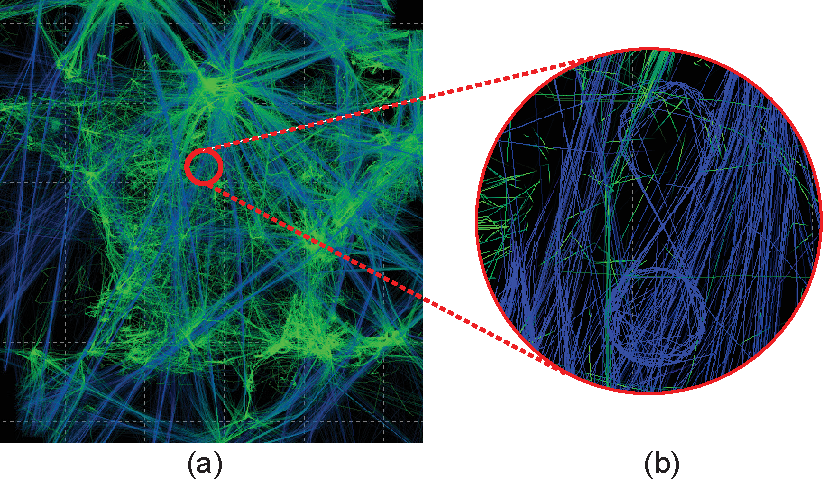
\includegraphics [width=0.45\textwidth]{images/aircraft.pdf} 
\caption{ Standard visualization of one day of recorded aircraft trajectories over France.\cite{hurter2009fromdady}. (a) An unusual trajectory is spotted but needs some manipulation to be unobstructed. (b) Zoom and color filtering technique to visualize abnormal trajectory of one aircraft performing a loop with an eight shape trajectory. This aircraft corresponds to a tanker waiting for refueling other aircraft.}
\label{f:fromdady}
\end{figure}
Figure \autoref{f:fromdady}-a shows one day of recorded aircraft trajectories and \autoref{f:fromdady}(b) shows a subset of such dataset where one can visualize an abnormal aircraft trajectory. A tanker aircraft performed an eight shape loop while waiting to refuel other aircraft. Even if the visualization of such specific trajectory is possible with existing tools, it remains a difficult task which requires time and complex settings. With our technique (with a volume size of 500x500x500), the user can easily spot the corresponding aircraft and even if this trajectory remains barely visible, our lens tools will remove the occluding trajectory thus providing a suitable point of view to fully investigate this trajectory. Furthermore, this obstruction free lens allows to look around the targeted trajectory in order to look for neighboring trajectories.

\begin{figure} 
\includegraphics [width=0.36\textwidth]{images/topViewFR.png} 
\includegraphics [width=0.4\textwidth]{images/VerticalViewLabel.png} 
\caption{Visualization of one day of recorded aircraft trajectories over France using our volume rendering framework. (a) The trajectories almost draw the map of France. (b) The trajectories are displayed according to their altitudes. }
\label{f:aircraft_orientation}
\end{figure}


